\section{Anhang}

\subsection*{Notenfolgen C - F Kapitel 2}

\begin{figure}[htbp] \centering
	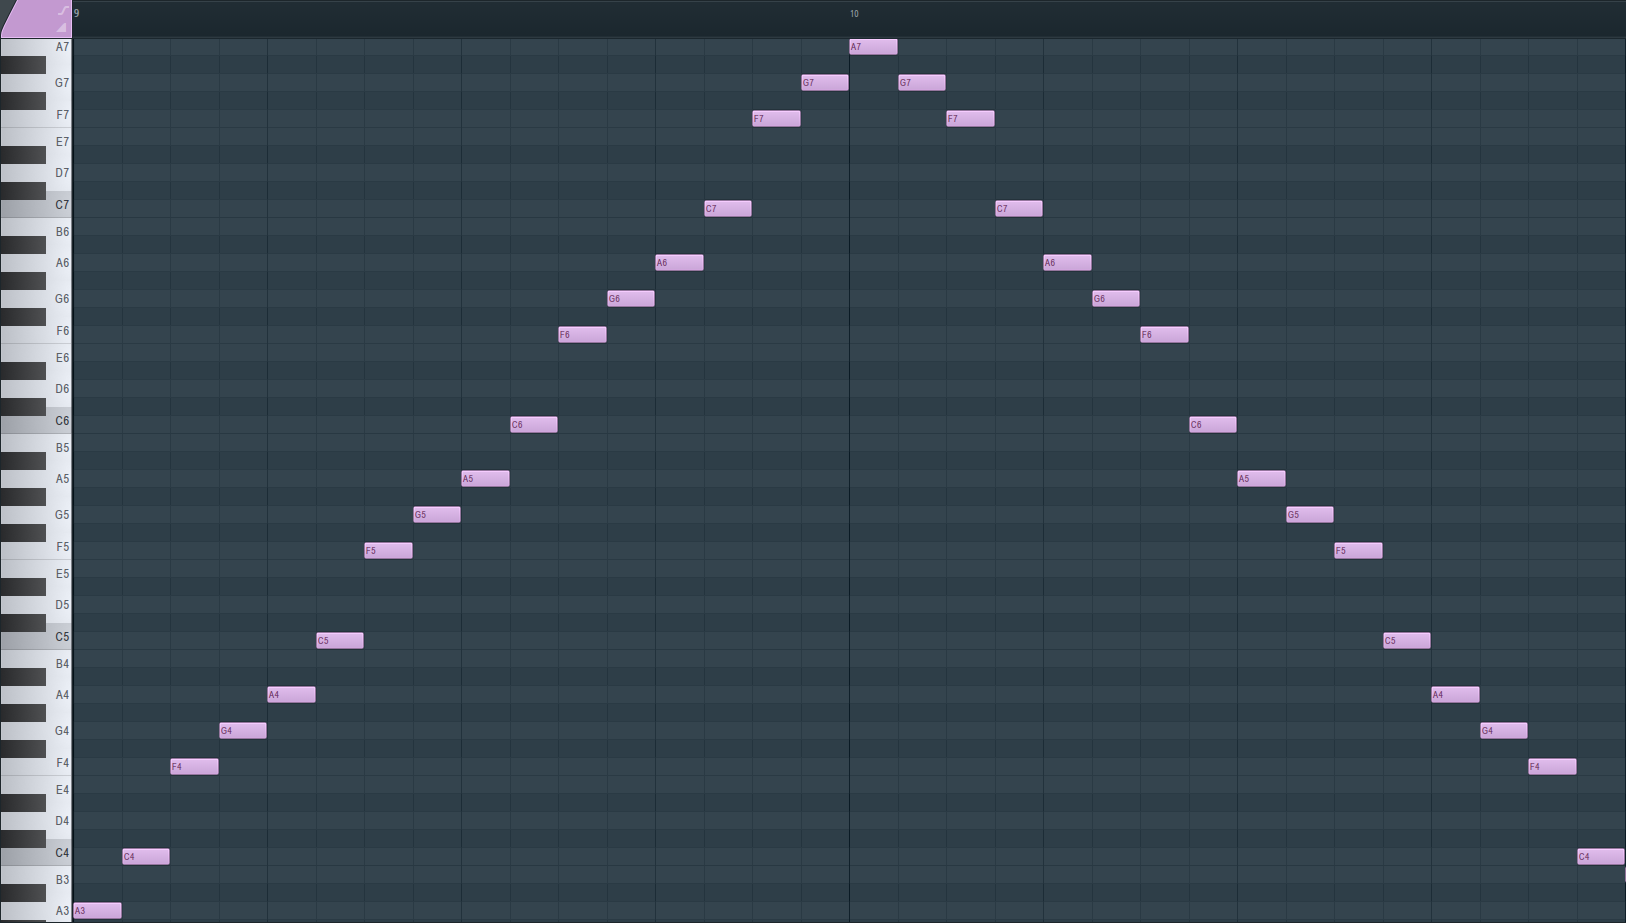
\includegraphics[width=.95\linewidth]{images/Noten_C.png}
	\caption{Notenabfolge C}
	\label{NotenabfolgeC}
\end{figure}

\begin{figure}[htbp] \centering
	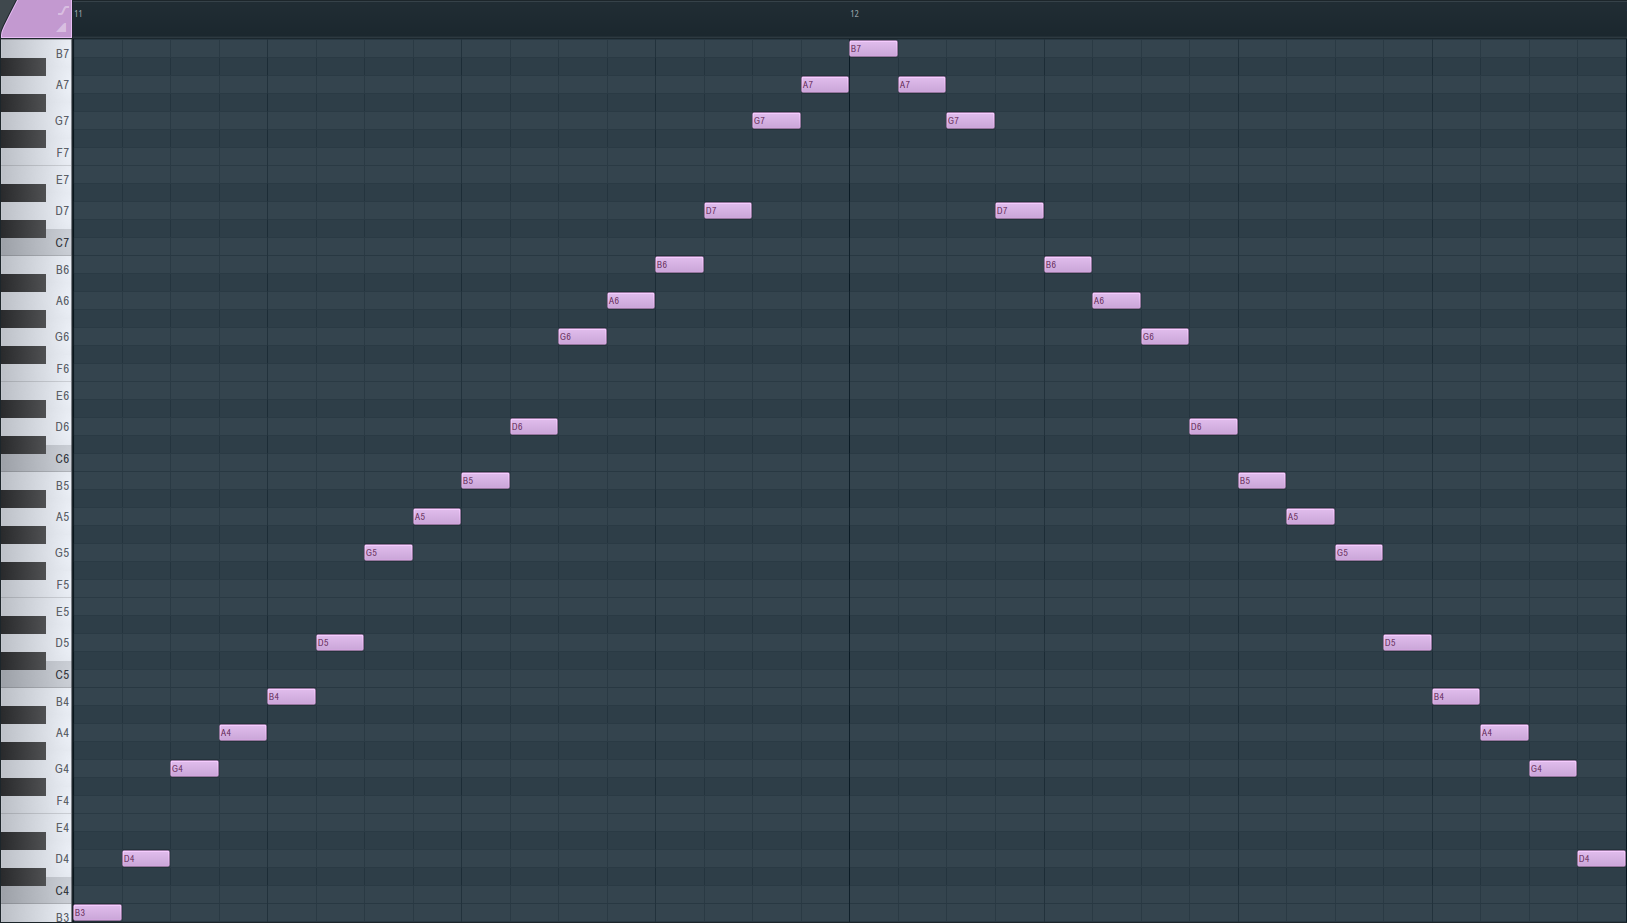
\includegraphics[width=.95\linewidth]{images/Noten_D.png}
	\caption{Notenabfolge D}
	\label{NotenabfolgeD}
\end{figure}

\begin{figure}[htbp] \centering
	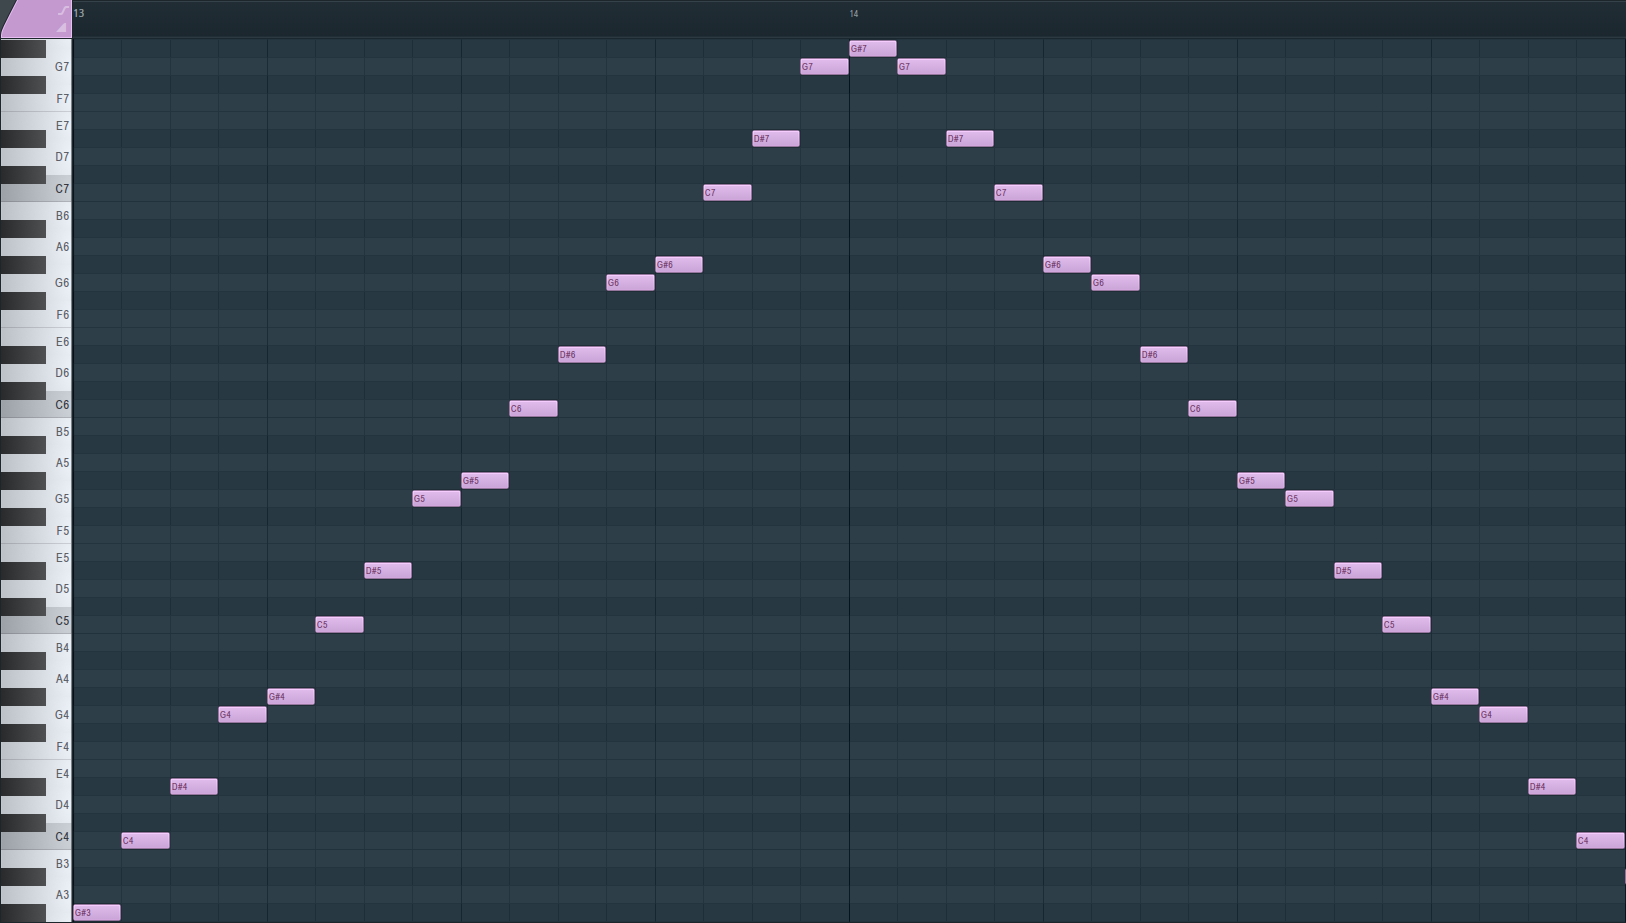
\includegraphics[width=.95\linewidth]{images/Noten_E.png}
	\caption{Notenabfolge E}
	\label{NotenabfolgeE}
\end{figure}

\begin{figure}[htbp] \centering
	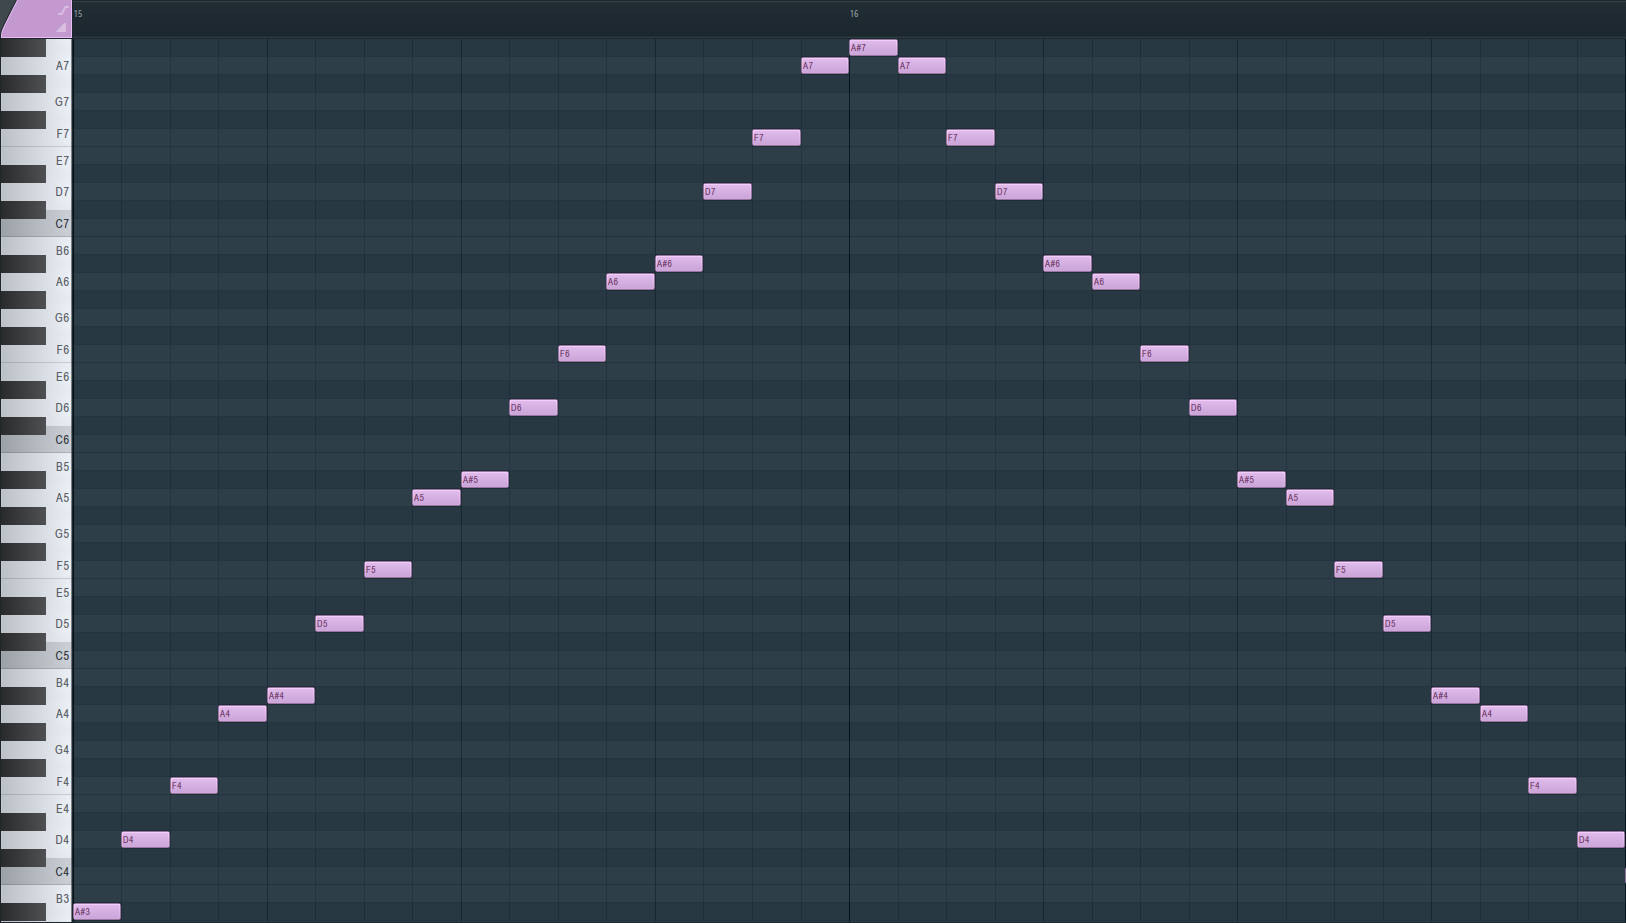
\includegraphics[width=.95\linewidth]{images/Noten_F.png}
	\caption{Notenabfolge F}
	\label{NotenabfolgeF}
\end{figure}


\begin{table}[htbp]
	\centering
	\begin{tabularx}{4.5cm}{|l|X|}
		\hline
		\$C0 & Ganze Note \\
		\hline
		\$80 & Ganze Triole \\
		\hline
		\$60 & Halbe Note \\
		\hline
		\$40 & Halbe Triole \\
		\hline
		\$30 & Viertelnote \\
		\hline
		\$20 & Viertel Triole \\
		\hline
		\$18 & Achtelnote \\
		\hline
		\$10 & Achtel Triole \\
		\hline
		\$0C & 16tel Note \\
		\hline
		\$09 & 16tel Triole \\
		\hline
		\$06 & 32tel Note \\
		\hline
		\$04 & 32tel Triole \\
		\hline
		\$03 & 64tel Note \\
		\hline
		\$02 & 64tel Triole \\
		\hline
	\end{tabularx}
	\caption{Längen in Hexwerte}
\end{table}

